% !TeX program = xelatex
\documentclass[acmsmall,screen,review,anonymous]{acmart}

\setcopyright{none}
\copyrightyear{2027}
\acmYear{2027}
\acmDOI{}
\acmConference[FSE 2027]
  {The ACM International Conference on the Foundations of Software Engineering}
  {July 12--16, 2027}
  {Shenzhen, China}
\acmISBN{}

\usepackage[ruled,vlined,linesnumbered]{algorithm2e}
\usepackage{array}
\usepackage{placeins}
\usepackage{tikz}
\usetikzlibrary{automata,positioning,arrows.meta}
\vbadness=10000

\usepackage{iftex}
\ifXeTeX\else
  \PackageError{main}{This manuscript requires XeLaTeX}%
    {Select XeLaTeX as the compiler, or keep the supplied latexmkrc file.}
\fi
\usepackage{xeCJK}
\IfFontExistsTF{Noto Serif CJK JP}{%
  \setCJKmainfont[
    ItalicFont=Noto Serif CJK JP,
    BoldItalicFont=Noto Serif CJK JP,
    SmallCapsFont=Noto Serif CJK JP
  ]{Noto Serif CJK JP}%
  \setCJKsansfont[
    ItalicFont=Noto Sans CJK JP,
    BoldItalicFont=Noto Sans CJK JP,
    SmallCapsFont=Noto Sans CJK JP
  ]{Noto Sans CJK JP}%
  \setCJKmonofont{Noto Sans Mono CJK JP}%
}{%
  \setCJKmainfont[
    BoldFont=ipaexg.ttf,
    ItalicFont=ipaexm.ttf,
    BoldItalicFont=ipaexg.ttf,
    SmallCapsFont=ipaexm.ttf
  ]{ipaexm.ttf}%
  \setCJKsansfont[
    BoldFont=ipaexg.ttf,
    ItalicFont=ipaexg.ttf,
    BoldItalicFont=ipaexg.ttf,
    SmallCapsFont=ipaexg.ttf
  ]{ipaexg.ttf}%
  \setCJKmonofont{ipaexg.ttf}%
}

\AtBeginDocument{%
  \providecommand\BibTeX{{Bib\TeX}}}

\newcommand{\Post}{\mathsf{Post}}
\newcommand{\Safe}{\mathsf{Safe}}
\newcommand{\Goal}{Q_{\mathrm{goal}}}
\newcommand{\rank}{\mathsf{rk}}
\newcommand{\ActT}{\mathsf{ActiveM}}
\newcommand{\Init}{\mathsf{Init}}
\newcommand{\Reach}{\mathsf{Reach}}
\newcommand{\SuccSet}{\mathsf{Succ}}
\newcommand{\En}{\mathsf{En}}
\newcommand{\Ev}{\mathsf{Ev}}
\newcommand{\Cand}{\mathsf{Cand}}
\newcommand{\Sigmauc}{\Sigma_{\mathrm{uc}}}
\newcommand{\Sigmac}{\Sigma_{\mathrm{c}}}
\newcommand{\SigmaN}{\Sigma_{\mathrm{N}}}
\newcommand{\SigmaU}{\Sigma_{\mathrm{upd}}}
\newcommand{\CLnew}{\mathsf{CL}^{\mathrm{new}}}
\newcommand{\ustart}[1]{\mathsf{start}(#1)}
\newcommand{\ustop}[1]{\mathsf{stop}(#1)}

% Derived from validated returned raw; elapsed/RSS are single-trial references, not medians.
\providecommand{\ADDirectFullWins}{14}
\providecommand{\ADDirectFullTimeouts}{13}
\providecommand{\ADWorkflowCapSeconds}{1200}
\providecommand{\ADWorkflowElapsedSeconds}{1201.7}
\providecommand{\ADWorkflowPeakRSSGiB}{13.9}
\providecommand{\ADPCCapSeconds}{3600}
\providecommand{\ADPCElapsedSeconds}{3605.2}
\providecommand{\ADPCPeakRSSGiB}{67.1}

% Generated from validated Xeon raw; do not edit.
\newcommand{\LFConditions}{21}
\newcommand{\LFFamilies}{8}
\newcommand{\LFPublishedWins}{21}
\newcommand{\LFForkWins}{16}
\newcommand{\LFSizeMatches}{15}
\newcommand{\LFSizeMismatches}{1}
\newcommand{\LFUnmeasured}{5}
\newcommand{\LFParserNM}{3}
\newcommand{\LFInstrumentationNM}{2}
\newcommand{\LFRailcabStateDelta}{5}
\newcommand{\LFRailcabTransitionDelta}{7}

% Derived elapsed-time bounds, never solver-only bounds.
\newcommand{\CensoredPairs}{12}
\newcommand{\CensoredBoundMin}{2.12}
\newcommand{\CensoredBoundMax}{910.06}

\providecommand{\RSMonitorOccurrences}{273}
\providecommand{\RSClassifiedOccurrences}{273}
\providecommand{\RSFluentDeterminedOccurrences}{0}
\providecommand{\RSExactOccurrences}{0}
\providecommand{\RSUntestedOccurrences}{273}
\providecommand{\RSUnclassifiedOccurrences}{0}
\providecommand{\RSNewOccurrences}{138}
\providecommand{\RSUpdateOccurrences}{135}
\providecommand{\RSAExactOccurrences}{138}
\providecommand{\RSEExactOccurrences}{0}
\providecommand{\RSAEUnverifiedOccurrences}{135}
\providecommand{\RSEObserverSyncOccurrences}{89}
\providecommand{\RSEResetConsistentOccurrences}{135}
\providecommand{\RSEAHExactOccurrences}{89}
\providecommand{\RSAHEUnverifiedOccurrences}{46}
\providecommand{\RSAInclusionNew}{138}
\providecommand{\RSAExactNew}{138}
\providecommand{\RSEExactUpd}{89}
\providecommand{\RSUpdOccurrences}{135}
\providecommand{\RSAUnverifiedNew}{0}
\providecommand{\RSEUnverifiedUpd}{46}

\begin{document}
\title{Fine-Grained Dynamic Update Controller Synthesis}

\author{Anonymous Author(s)}
\renewcommand{\shortauthors}{Anonymous Author(s)}

\begin{abstract}
Updating a running controlled system creates a mixed-version interval beyond the old and new controllers' separate safety guarantees. Components may become ready for replacement at different times, with requirements active across different intervals. Fine-Grained Dynamic Update Controller Synthesis (FG-DUCS) combines set-valued component transfer, requirement lifetimes and residuals, precedence, and compatible handover targets. Update commands and handover require uncontrollable quiescence.

We encode the problem as a finite reachability game and specialize its attractor computation with lazy successor generation. The terminating, sound and complete procedure certifies all entries/outcomes of the supplied finite model; execution guarantees are conditional on residual soundness (RS) and runtime assumptions A1--A4. It returns a policy/rank/handover certificate or a losing region. For the benchmark inputs, residual soundness is mechanically established for all \RSAExactNew{} new-requirement initializations and \RSEExactUpd{} of \RSUpdOccurrences{} update-time initializations under the stated interpretations; the remaining \RSEUnverifiedUpd{} reference action predicates and are unverified. Witnesses separate fine-grained from bulk updates and $K+1$ discovered states from $2^K$ under full expansion. Raw-LTS expectations agree with 92 correctness and 14 capability jobs. On 27 instances from nine DUCS benchmarks, with a 64~GiB heap and 20-minute budget, FG-DUCS-OTF decides 26: 25 realizable and one unrealizable with a checked losing certificate. Explicit same-semantics solving decides 14 and takes $1.6$--$2{,}124\times$ longer on their paired five-run medians; the fork's legacy synthesis path decides nine. Five legacy cells are unmeasured due to an author-side capture cap. On 90 hub games, paired median speedups are $5.3$--$118\times$; Travel models expose a shared resource limit at six or more concurrent agencies. Resource-limited cells remain unresolved.
\end{abstract}

\begin{CCSXML}
<ccs2012>
 <concept>
  <concept_id>10011007.10011074.10011092</concept_id>
  <concept_desc>Software and its engineering~Software evolution</concept_desc>
  <concept_significance>500</concept_significance>
 </concept>
</ccs2012>
\end{CCSXML}

\ccsdesc[500]{Software and its engineering~Software evolution}
\keywords{dynamic software updating, discrete-event controller synthesis, supervisory control, on-the-fly synthesis}

\maketitle

\section{Introduction}
\label{sec:introduction}

A deployed controlled system must evolve while its environment continues to act. A production cell may still hold a workpiece when its controller or equipment model changes; a workflow may have obligations left by an earlier request. Stopping operation can postpone the update, but separate verification of the old and new configurations does not explain how to move safely between them. Runtime evolution therefore needs a controller for the transition itself, connecting the assurance of stable configurations to the behavior permitted during change~\cite{Cheng2009SASRoadmap,Andersson2013SEAMSProcesses,Giuffrida2013SafeLiveUpdate,Sokolowski2022DynamicWorkflowUpdates}.

Reconfiguration connects valid configurations through safe intermediate states~\cite{KramerMagee1990Quiescence,CoullonEtAl2024Survey}; control may change with assumptions and goals~\cite{DIppolito2014MultiTierControl}. State-transformer synthesis~\cite{ZhaoEtAl2021ObjectTransformers}, combined-version verification~\cite{HaydenEtAl2012DSUCorrectness} and distributed version consistency~\cite{BaresiEtAl2017VersionConsistency} address complementary concerns. We synthesize control between supplied transfers.

Components can become replaceable at different times, for example after releasing a resource. Requirements also have different lifetimes: old protection may remain necessary until replacement, while a new requirement inherits an obligation from the current state. Dynamic scenario updates expose such intermediate obligations~\cite{Ghezzi2012DynamicScenarioUpdate,PanzicaLaManna2013CorrectnessDynamicUpdates}. Synthesis must coordinate changes, ordinary operation and requirement boundaries throughout this interval.

Dynamic Update Controller Synthesis (DUCS) synthesizes control preserving safety and completing an update~\cite{Nahabedian2016SEAMS,Nahabedian2020}. Its native interface offers global environment reconfiguration and whole-set stop/start. Transfers may be set-valued; intermediate steps can be encoded in the new environment, and transition requirements permit specification overlap~\cite[Sec.~4.2]{Nahabedian2020}. Individual component/requirement boundaries need additional encoding. The GR(1) bridge similarly uses a switching condition~\cite{Amram2022GR1DynamicUpdate}. We make these finer decisions explicit inputs and synthesize their order and outcome-dependent continuation.

FG-DUCS takes verified old/new closed loops, component transfer relations, individual requirement boundaries and residuals, precedence, and handover targets. Commands and handover require uncontrollable quiescence. In the Production Cell below, replacing the empty station, moving the product, and replacing the other station succeeds although no reachable state permits both replacements together.

Three difficulties remain: transfer outcomes can require different continuations; independent changes induce exponentially many configurations; and success must cover every reachable old-state entry and permitted outcome. FG-DUCS encodes a finite reachability game and explores successors lazily, returning a policy with decreasing ranks and compatible handover targets, or a losing region.

Strong planning and on-the-fly games provide the algorithmic foundation~\cite{Cimatti1998StrongPlanning,TripakisAltisen1999,CiolekEtAl2023OTFDCS}. We contribute the update contract and encoding, lazy buckets, certificates and evaluation. The preliminary O-DUCS report explores updates from old reachable states~\cite{HiranoEtAl2024ODUCS}; FG-DUCS develops component/requirement boundaries and a terminating, sound and complete certifying procedure.

\paragraph{Contributions}
\begin{itemize}
\item \textbf{C1: Fine-grained formulation.} A finite contract combines set-valued component transfers, requirement lifetimes and residuals, precedence, and handover targets. Complete witnesses separate three granularity restrictions (Section~\ref{sec:mechanism-boundary}).
\item \textbf{C2: Certifying on-the-fly synthesis.} A terminating, sound, complete solver covers all roots/outcomes and returns a WIN certificate $(\sigma,\rank,\kappa)$ or LOSS certificate $L$ (Theorem~\ref{thm:correctness}).
\item \textbf{C3: Search separation.} An independent-update family requires $K+1$ discovered states for lazy exploration and $2^K$ for Direct-Full, isolating successor-generation cost.
\item \textbf{C4: Evaluation.} Raw-LTS checks validate decisions. On 27 Xeon instances, lazy synthesis decides 26 versus Direct-Full's 14 and reduces paired median time by $1.6$--$2{,}124\times$. Hub tests yield paired speedups of $5.3$--$118\times$; Travel exposes shared resource limits.
\end{itemize}
Guarantees are relative to the supplied finite model and RS; execution additionally assumes A1--A4. Benchmark residual guarantees use the scoped requirement meanings defined in Section~3.1 and Supplement~S3.

\section{Motivating Example}
\label{sec:example}
% Complete W_cell diagram. Wedge records are checked against executable primitives.
\begin{figure*}[!htbp]
\centering
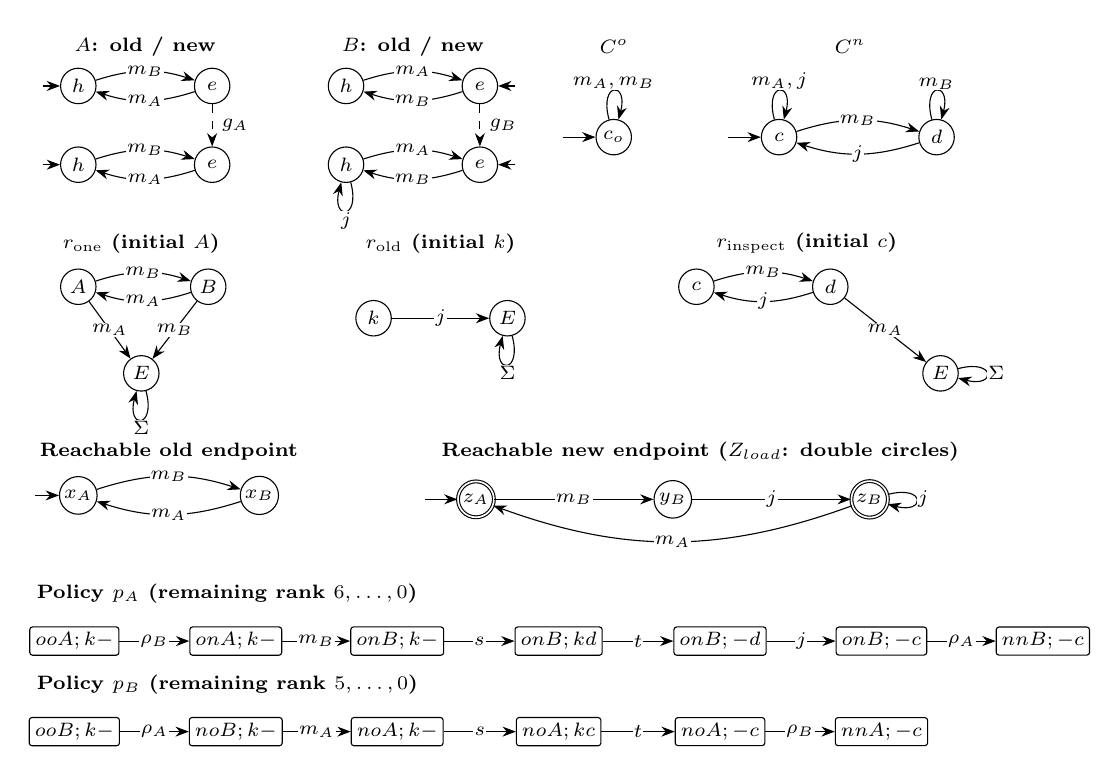
\begin{tikzpicture}[>=Stealth, every node/.style={font=\scriptsize},
 st/.style={circle,draw,minimum size=4.5mm,inner sep=1pt},
 ps/.style={draw,rounded corners=1pt,inner sep=2pt,font=\scriptsize},
 lab/.style={font=\scriptsize\bfseries}]
\newcommand{\FGedge}[5]{\draw[->,#5] (#1-#2) to node[font=\scriptsize,fill=white,inner sep=.4pt] {$#3$} (#1-#4);}
\node[lab] at (1.35,.5) {$A$: old / new};
\node[st] (Ao-h) at (.5,0) {$h$}; \node[st] (Ao-e) at (2.2,0) {$e$};
\node[st] (An-h) at (.5,-1.0) {$h$}; \node[st] (An-e) at (2.2,-1.0) {$e$};
\draw[->] (.05,0)--(Ao-h); \draw[->] (.05,-1)--(An-h);
\FGedge{Ao}{h}{m_B}{e}{bend left=18}
\FGedge{Ao}{e}{m_A}{h}{bend left=18}
\FGedge{An}{h}{m_B}{e}{bend left=18}
\FGedge{An}{e}{m_A}{h}{bend left=18}
\draw[->,dashed] (Ao-e)--node[right] {$g_A$}(An-e);
\node[lab] at (4.75,.5) {$B$: old / new};
\node[st] (Bo-h) at (3.9,0) {$h$}; \node[st] (Bo-e) at (5.6,0) {$e$};
\node[st] (Bn-h) at (3.9,-1) {$h$}; \node[st] (Bn-e) at (5.6,-1) {$e$};
\draw[->] (6.05,0)--(Bo-e); \draw[->] (6.05,-1)--(Bn-e);
\FGedge{Bo}{e}{m_B}{h}{bend left=18}
\FGedge{Bo}{h}{m_A}{e}{bend left=18}
\FGedge{Bn}{e}{m_B}{h}{bend left=18}
\FGedge{Bn}{h}{m_A}{e}{bend left=18}
\FGedge{Bn}{h}{j}{h}{loop below}
\draw[->,dashed] (Bo-e)--node[right] {$g_B$}(Bn-e);
\node[lab] at (7.3,.5) {$C^o$};
\node[st] (Co-co) at (7.3,-.65) {$c_o$};\draw[->] (6.65,-.65)--(Co-co);
\FGedge{Co}{co}{m_A,m_B}{co}{loop above}
\node[lab] at (10.3,.5) {$C^n$};
\node[st] (Cn-c) at (9.4,-.65) {$c$};\node[st] (Cn-d) at (11.4,-.65) {$d$};
\draw[->] (8.75,-.65)--(Cn-c);
\FGedge{Cn}{c}{m_A,j}{c}{loop above}
\FGedge{Cn}{c}{m_B}{d}{bend left=18}
\FGedge{Cn}{d}{j}{c}{bend left=18}
\FGedge{Cn}{d}{m_B}{d}{loop above}
\node[lab] at (1.3,-2) {$r_{\rm one}$ (initial $A$)};
\node[st] (One-A) at (.5,-2.55) {$A$};\node[st] (One-B) at (2.15,-2.55) {$B$};\node[st] (One-E) at (1.3,-3.65) {$E$};
\FGedge{One}{A}{m_B}{B}{bend left=18}
\FGedge{One}{B}{m_A}{A}{bend left=18}
\FGedge{One}{A}{m_A}{E}{}
\FGedge{One}{B}{m_B}{E}{}
\FGedge{One}{E}{\Sigma}{E}{loop below}
\node[lab] at (5.1,-2) {$r_{\rm old}$ (initial $k$)};
\node[st] (Old-k) at (4.25,-2.95) {$k$};\node[st] (Old-E) at (5.95,-2.95) {$E$};
\FGedge{Old}{k}{j}{E}{}
\FGedge{Old}{E}{\Sigma}{E}{loop below}
\node[lab] at (9.75,-2) {$r_{\rm inspect}$ (initial $c$)};
\node[st] (Ins-c) at (8.35,-2.55) {$c$};\node[st] (Ins-d) at (10.05,-2.55) {$d$};\node[st] (Ins-E) at (11.45,-3.65) {$E$};
\FGedge{Ins}{c}{m_B}{d}{bend left=18}
\FGedge{Ins}{d}{j}{c}{bend left=18}
\FGedge{Ins}{d}{m_A}{E}{}
\FGedge{Ins}{E}{\Sigma}{E}{loop right}
\node[lab] at (1.65,-4.65) {Reachable old endpoint};
\node[st] (OldCL-xA) at (.5,-5.2) {$x_A$};\node[st] (OldCL-xB) at (2.8,-5.2) {$x_B$};
\draw[->] (-.05,-5.2)--(OldCL-xA);
\FGedge{OldCL}{xA}{m_B}{xB}{bend left=18}
\FGedge{OldCL}{xB}{m_A}{xA}{bend left=18}
\node[lab] at (8.4,-4.65) {Reachable new endpoint ($Z_{load}$: double circles)};
\node[st,double] (NewCL-zA) at (5.55,-5.25) {$z_A$};\node[st] (NewCL-yB) at (8.05,-5.25) {$y_B$};\node[st,double] (NewCL-zB) at (10.55,-5.25) {$z_B$};
\draw[->] (4.9,-5.25)--(NewCL-zA);
\FGedge{NewCL}{zA}{m_B}{yB}{}
\FGedge{NewCL}{yB}{j}{zB}{}
\FGedge{NewCL}{zB}{m_A}{zA}{bend left=20}
\FGedge{NewCL}{zB}{j}{zB}{loop right}
\node[lab,anchor=west] at (-.15,-6.45) {Policy $p_A$ (remaining rank $6,\ldots,0$)};
\foreach \n/\txt in {0/ooA;k-,1/onA;k-,2/onB;k-,3/onB;kd,4/onB;-d,5/onB;-c,6/nnB;-c}
 \node[ps] (PA-\n) at ({.45+2.05*\n},-7.05) {$\txt$};
\FGedge{PA}{0}{\rho_B}{1}{}
\FGedge{PA}{1}{m_B}{2}{}
\FGedge{PA}{2}{s}{3}{}
\FGedge{PA}{3}{t}{4}{}
\FGedge{PA}{4}{j}{5}{}
\FGedge{PA}{5}{\rho_A}{6}{}
\node[lab,anchor=west] at (-.15,-7.6) {Policy $p_B$ (remaining rank $5,\ldots,0$)};
\foreach \n/\txt in {0/ooB;k-,1/noB;k-,2/noA;k-,3/noA;kc,4/noA;-c,5/nnA;-c}
 \node[ps] (PB-\n) at ({.45+2.05*\n},-8.2) {$\txt$};
\FGedge{PB}{0}{\rho_A}{1}{}
\FGedge{PB}{1}{m_A}{2}{}
\FGedge{PB}{2}{s}{3}{}
\FGedge{PB}{3}{t}{4}{}
\FGedge{PB}{4}{\rho_B}{5}{}
\end{tikzpicture}
\par\smallskip
\fbox{\parbox{\dimexpr\linewidth-2\fboxsep-2\fboxrule\relax}{\scriptsize
$m_A/m_B/j=move_A/move_B/inspect$; $o/n,h/e,k/c/d/E/-=$ old/new, holding/empty, ok/clear/pending/error/inactive.
$\SigmaN=\{m_A,m_B,j\}$, $\SigmaU=\{\rho_A,\rho_B,s,t\}$, $\Sigmauc=\emptyset$; $s=\ustart{r_{inspect}}\prec t=\ustop{r_{old}}$.
For $v_Av_Bx;\mu_o\mu_i$, $P=\{\rho_i:v_i=o\}\cup\{s:\mu_i=-\}\cup\{t:\mu_o\ne-\}$; $x$ is holder and $r_{one}$ state.
Initial plant states are $(A_h^v,B_e^v)$. Alphabets are the displayed outgoing labels over all local states; $g_i=\{(e_i^o,e_i^n)\}$.
\par $R^{old/new/upd}=\{r_{old}\}/\{r_{inspect}\}/\{r_{one}\}$.
$\mathsf{Start}_{one}$ is the two old one-product states, $\iota_{one}=$ holder; its observation preserves moves (exact RS).
$\mathsf{Start}_{inspect}$ contains all eight tagged one-product states; $\iota_{inspect}=d$ at $B_h$, otherwise $c$.
Before activation, its observation erases every label except $s$. Thus $c$ is exact at $B_e$; at $B_h$, $\mathcal L(d)\subsetneq\mathcal L(c)$ (witness $m_A$), a conservative residual.
\par $x_A=(A_h^o,B_e^o,c_o,k)$, $x_B=(A_e^o,B_h^o,c_o,k)$;
$z_A=(A_h^n,B_e^n,c,c)$, $y_B=(A_e^n,B_h^n,d,d)$, $z_B=(A_e^n,B_h^n,c,c)$.
$Q_0$ consists of the first states of $p_A,p_B$; their last states are goals with $\kappa=z_B,z_A$, respectively; $Z_{load}=\{z_A,z_B\}$.
The displayed paths define $\sigma$ (empty elsewhere), with 13 states and 11 edges. A bulk $g_A\times g_B$ requires unreachable $(A_e^o,B_e^o)$.
\par Unlisted plant/controller transitions are empty; unlisted non-error monitor transitions self-loop; $E$ absorbs every label. Comma-separated arrow labels denote separate edges. The four $\Post$ rules determine every bucket; the unsafe-inclusive closure census is in Supplement~S1.
}}
\caption{Complete Production Cell witness $\mathcal W_{\rm cell}$: local replacements, active requirements, endpoints and a policy from both entries. Dashed arrows are transfer relations, not ordinary events.}
\Description{Four two-state plant versions, three monitors including every error edge, old and new controllers and endpoints, and two labeled policy chains. The legend supplies the full update contract and omitted-transition conventions.}
\label{fig:wcell-complete}
\end{figure*}


Consider a finite Production Cell witness with two stations, $A$ and $B$, sharing exactly one product~\cite{Lewerentz1995ProductionCell,Nahabedian2020}. The product must be neither lost nor duplicated, and a station holding it cannot be replaced. Write $h/e$ for holding/empty and $o/n$ for old/new. The old controller moves the product between $(A_h^o,B_e^o)$ and $(A_e^o,B_h^o)$. An update may be requested at either state, so one synthesized policy must handle both entries.

A bulk transfer applies both local transfer relations together. Each relation accepts only an empty station, so their product requires $(A_e^o,B_e^o)$. This state is unreachable while preserving one product. Waiting for a different old state cannot make bulk replacement possible. With separate transfer events, the entry with $A$ holding instead admits
\[
(A_h^o,B_e^o)\xrightarrow{\rho_B}(A_h^o,B_e^n)
\xrightarrow{move_B}(A_e^o,B_h^n)
\xrightarrow{\rho_A}(A_e^n,B_h^n).
\]
The initially empty $B$ is replaced first; moving the product then makes $A$ replaceable. The symmetric entry reverses the component order. This component projection is only part of the update: the requirements determine where the remaining boundary and inspection events belong.

The interval monitor $r_{\rm one}$ tracks the holder throughout. Old $r_{\rm old}$ forbids inspection until its own stop, while new $r_{\rm inspect}$ requires inspection before the product next leaves $B$. After the first transfer and product move, $A$ is old, $B$ is new and holding, and $r_{\rm old}$ is still active. Starting $r_{\rm inspect}$ at this point installs its pending-obligation state $d$, rather than the initial clear state $c$. This is the role of residual initialization $\iota$: activation must use a monitor state appropriate to the supplied history meaning. The precedence $start(r_{\rm inspect})\prec stop(r_{\rm old})$ creates a brief overlap; stopping the old prohibition then permits inspection and discharges the pending obligation. Figure~\ref{fig:wcell-complete} specifies the complete fixture and both policy paths; Section~\ref{sec:mechanism-boundary} proves the separation.

The returned policy tells an update orchestrator which controllable event to permit at each observed state. Its rank certifies finite progress for every modeled outcome, and its handover table identifies the compatible new-controller state to load. A LOSS region identifies an obstruction to the supplied contract, providing a concrete basis for revising that contract.

We connect this small witness to nine DUCS-derived benchmark models in Section~\ref{sec:evaluation}. In Industry/R1, a checked losing region exposes the need for a validation step forbidden during the update. Permitting that event in a separate contract variant makes the update realizable; Section~\ref{sec:evaluation} preserves both the original LOSS and the variant result.

\FloatBarrier

\section{FG-DUCS}
\label{sec:formalization}

Let $v\in\{\mathrm{old},\mathrm{new}\}$ denote the two versions. Each supplied closed loop $E^v\parallel C^v$ is separately verified against $R^v$; $\mathsf{CL}^v$ instruments it with monitors. FG-DUCS controls the intervening component and requirement changes. Execution interpretation uses A1--A4 in Section~\ref{sec:runtime-boundary}.

\subsection{System, Requirement, and Update Inputs}

\paragraph{Finite LTSs and safety monitors}
An LTS is $\mathcal L=(S,\Sigma_{\mathcal L},\delta,s^0)$, where
$\delta:S\times\Sigma_{\mathcal L}\to2^S$ permits nondeterministic outcomes. Partition the global event set as
$\Sigma=\Sigmauc\uplus\Sigmac$, where events in $\Sigmauc$ cannot be disabled. In a synchronous product, an event shared by components synchronizes only when every component having that event can take it; nonparticipating components retain their states~\cite{MageeKramer2006}.
Only components generate events; controllers and monitors neither generate them nor select outcomes. A safety requirement $r$ has a distinct total deterministic monitor $t_r=(M_r,\Sigma,\eta_r,m_r^0,F_r)$, whose absorbing errors recognize violating prefixes~\cite{AlpernSchneider1985,KupfermanVardi2001}. Write $\mathbb T_R=\{t_r:r\in R\}$ and $F_t$ for the error states of monitor $t$; an empty monitor product is a one-state error-free LTS. Monitors observe labels, whereas policies also observe successor states. Outcome-sensitive safety therefore requires distinguishing labels.

\begin{definition}[Typed FG-DUCS update contract]
\label{def:fg-inputs}
\label{def:update_plan}
\emph{Component-level state transfer.}
For each $i\in I$, let $e_i^{\mathrm{old}},e_i^{\mathrm{new}}$ be the pre-update and post-update components and let $g_i\subseteq S_{e_i^{\mathrm{old}}}\times S_{e_i^{\mathrm{new}}}$ be their state-transfer relation.
  Define $g_i(s)=\{s'\mid(s,s')\in g_i\}$. The supplied $g_i$ includes every modeled outcome of transformation, activation and rewiring. Let $E^v=\mathop{\parallel}_{i\in I}e_i^v$. Each component state carries its old/new version tag.

\par\noindent\emph{Requirement active periods and monitor initialization.}
Let pairwise-disjoint $R^{\mathrm{old}},R^{\mathrm{new}},R^{\mathrm{upd}}$ contain the pre-update, post-update, and update-interval safety requirements, respectively.
Old monitors inherit their monitored endpoint states at admission. For each $r\in R^{\mathrm{new}}\cup R^{\mathrm{upd}}$, rather than resetting away history, the input supplies a set $\mathsf{Start}_r$ of version-tagged component tuples and a \emph{monitor-initialization map} $\iota_r:\mathsf{Start}_r\to M_r\setminus F_r$.
Residual-sound initialization requires
  \[
    \mathcal L_r(\iota_r(\xi))\subseteq\mathcal C_r(\xi)
    \quad(\xi\in\mathsf{Start}_r).
    \tag{RS}\label{eq:residual-soundness}
  \]
Here $\mathcal L_r$ is the initialized monitor's safe continuation language and $\mathcal C_r$ the continuations compatible with every supplied activation history at $\xi$. RS concerns the supplied requirement/observation meanings; Supplement~S3.1 distinguishes history-inclusive H, activation-safe A and entry-scoped E meanings and their exactness conditions. Unverified cases retain RS as an external premise. For $r\in R^{\mathrm{upd}}$, $\mathsf{Start}_r$ includes every reachable old component state.

\par\noindent\emph{Verified pre-update and post-update closed loops and admissible handover targets.}
\label{def:endpoint_controllers}
For $v\in\{\mathrm{old},\mathrm{new}\}$, finite $C^v$ preserves uncontrollables and makes $E^v\parallel C^v$ deadlock-free and satisfy every requirement in $R^v$. After hiding controller auxiliary events, its observation alphabet is $\bigcup_i\Sigma_{e_i^v}$. Their union over both versions is the ordinary alphabet $\SigmaN$. The monitored endpoints are
  \[
  \mathsf{CL}^{\mathrm{old}}:=E^{\mathrm{old}}\parallel C^{\mathrm{old}}\parallel\mathop{\parallel}_{r\in R^{\mathrm{old}}}t_r,
  \qquad
  \CLnew:=E^{\mathrm{new}}\parallel C^{\mathrm{new}}\parallel\mathop{\parallel}_{r\in R^{\mathrm{new}}}t_r
  \]
Write $\Reach$ for initial-state reachability. Supply nonempty $Z_{\mathrm{load}}\subseteq\Reach(\CLnew)$ as the handover set, including component, new-controller and new-monitor states. Target reachability is checked.

\par\noindent\emph{One-shot update events and dependencies.}
The set of update events, each executed exactly once, is
  \[
  \SigmaU=
    \{\rho_i\mid i\in I\}
    \cup\{\ustop{r}\mid r\in R^{\mathrm{old}}\}
    \cup\{\ustart{r}\mid r\in R^{\mathrm{new}}\}.
  \tag{1}
  \]
The events $\rho_i,\ustop{r},\ustart{r}$ respectively update a component, deactivate a pre-update requirement monitor, and activate a post-update requirement monitor. Update events are distinct controllable events disjoint from ordinary events $\SigmaN$; that is,
$\Sigma=\SigmaN\uplus\SigmaU$ and $\SigmaU\subseteq\Sigmac$. Even after choosing $\rho_i$, the controller cannot choose the outcome in $g_i$; it is one model transition.
Update events use the non-preemptive successor rule in Definition~\ref{def:successor}: they are enabled only when no uncontrollable ordinary event is enabled.

Let the strict partial order $\prec\ \subseteq\SigmaU\times\SigmaU$ express precedence among update operations. For a pending-event set $P$, event $a$ is order-enabled exactly when $a\in P$ and every $a'\prec a$ has left $P$.
Monitors self-loop on update events that they do not specify.
\par\noindent\emph{Eligibility.}
Eligibility checks the finite input's types, event ownership, controllability and monitor structure; safe, deadlock-free endpoint controllers that preserve uncontrollables; complete update-monitor entry domains; strict partial-order dependencies; and reachable load targets. RS is external evidence for the supplied initialization meanings. Supplement~S2.1 gives every check; synthesis checks initialization types, domains and non-error values, while activation-history completeness remains an input obligation.
\end{definition}

Put an interval-wide property in $R^{\mathrm{upd}}$ and one required after handover in $R^{\mathrm{new}}$; to overlap new and old protection, require $\ustart{r^{\mathrm{new}}}\prec\ustop{r^{\mathrm{old}}}$.

\subsection{Update States and Transitions}

\begin{definition}[Update game induced by the contract]
\label{def:configuration}
\label{def:init}
\emph{States and all entry states.}
An update state is a triple $q=(\xi,\mu,P)$.
The set $P\subseteq\SigmaU$ contains the pending events, and
\[
 \xi(i)\in
 \{\mathrm{old}\}\times S_{e_i^{\mathrm{old}}}
 \ \uplus\
 \{\mathrm{new}\}\times S_{e_i^{\mathrm{new}}},
 \qquad
 \rho_i\in P\Longleftrightarrow
 \xi(i)\in\{\mathrm{old}\}\times S_{e_i^{\mathrm{old}}}.
\tag{2}\label{eq:version-invariant}
\]
$\mu$ stores states for $\mathbb T=\mathbb T_{R^{\mathrm{old}}}\cup
\mathbb T_{R^{\mathrm{new}}}\cup\mathbb T_{R^{\mathrm{upd}}}$, with
$\mu(t_r)\in M_r\cup\{\bot\}$ for each $t_r\in\mathbb T$. $\bot$ denotes inactivity and belongs to no $M_r$.
The set of active monitors is
\[
\ActT(P)=
\mathbb T_{R^{\mathrm{upd}}}
\cup\{t_r\mid r\in R^{\mathrm{old}},\,\ustop{r}\in P\}
\cup\{t_r\mid r\in R^{\mathrm{new}},\,\ustart{r}\notin P\},
\tag{3}
\]
and we require $t\in\ActT(P)\Longleftrightarrow\mu(t)\neq\bot$.

The function $\Init(z)$ inherits component state $\xi$ and pre-update monitor states from monitored pre-update closed-loop state $z$, leaves the post-update monitors inactive,
initializes the update-interval monitors using $\iota_r(\xi)$,
and sets $P=\SigmaU$. It does not inherit the $C^{\mathrm{old}}$ component of $z$, because update admission switches from the pre-update controller to the update orchestrator. The update-entry set is
\[
 Q_0=\{\Init(z)\mid
 z\in\Reach(\mathsf{CL}^{\mathrm{old}})\}.
\tag{4}\label{eq:initial}
\]
One policy covers all reachable old states; restricted admission is a different problem. For the cell, $q_A^0/q_B^0$ denote entry with $A/B$ holding the product, so $Q_0=\{q_A^0,q_B^0\}$.
\par\noindent\emph{Four kinds of implicit transitions.}
\label{def:successor}
For $q=(\xi,\mu,P)$ with $\xi(i)=(v,s)$, call $e_i^v$ the active local LTS of component $i$. Let $U(q)$ contain the uncontrollable ordinary events enabled by the active-component synchronous product (including events whose outcomes are unsafe). The ordinary-event rule below determines $U(q)$ independently of update events and goal recognition. For every $a\in\SigmaU$, impose
\[
 U(q)\ne\emptyset\quad\Longrightarrow\quad\Post(q,a)=\emptyset.
 \tag{NP}\label{eq:nonpreemption}
\]
When $U(q)=\emptyset$, the orchestrator may issue one enabled update command; the command occurs as one event with its outcome chosen from the full successor set. Define $\Post(q,a)$ to contain exactly the successors below, preserving every unstated component of $\xi,\mu,P$; ``advance $T$'' sets $\mu'(t)=\eta_t(\mu(t),a)$ for each $t\in T$.

\begin{description}
  \item[Ordinary event $a\in\SigmaN$.]
  If $a$ belongs to the local event set of at least one active component and every active component having $a$ can transition, take every synchronous-product outcome and advance $\ActT(P)$.

  \item[Component update $\rho_i$.]
  If $U(q)=\emptyset$, order-enabled, and $\xi(i)=(\mathrm{old},s)$, set $\xi'(i)=(\mathrm{new},s')$ for each $s'\in g_i(s)$, delete $\rho_i$ from $P$, and advance $\ActT(P)$.

  \item[Requirement deactivation $\ustop{r}$.]
  If $U(q)=\emptyset$ and order-enabled, advance $\ActT(P)\setminus\{t_r\}$, retain inactive monitors at $\bot$, set $\mu'(t_r)=\bot$, and delete $\ustop{r}$ from $P$; $t_r$ does not observe it.

  \item[Requirement activation $\ustart{r}$.]
  If $U(q)=\emptyset$, order-enabled, and $\xi\in\mathsf{Start}_r$, advance $\ActT(P)$, retain other inactive monitors at $\bot$, install $\mu'(t_r)=\iota_r(\xi)$, and delete $\ustart{r}$ from $P$; $t_r$ begins online observation afterward.
\end{description}
If a precondition is false, the successor set is empty; every nondeterministic outcome is included and environment-chosen.
Let $\mathcal Q$ be the least set containing $Q_0$ and closed under all $\Post$ transitions, and let $\En_{\mathrm{uc}}(q),\En_{\mathrm{c}}(q)$ be the sets of uncontrollable and controllable events, respectively, whose successor sets are nonempty.
\par\noindent\emph{Safety and handover-ready goals.}
\label{def:safe_goal}
An update state $q=(\xi,\mu,P)$ is safe when no active monitor is in an error state:
\[
 \Safe(q)\Longleftrightarrow
 \forall t\in\ActT(P):\mu(t)\notin F_t.
\tag{5}\label{eq:safe}
\]
For an update state $q$ with $P=\emptyset$ and a state $z\in Z_{\mathrm{load}}$, write $q\sim z$ when, component by component and monitor by monitor, the component states after removing the version tags and all post-update safety-monitor states agree between $q$ and $z$.
The handover map $\kappa$ supplies the new-controller state from its selected $z$.
Define the goal-state set as
\[
\Goal=\{q=(\xi,\mu,\emptyset)\in\mathcal Q\mid
\Safe(q)\land U(q)=\emptyset\land\exists z\in Z_{\mathrm{load}}:q\sim z\}.
\tag{6}\label{eq:goal}
\]
At a goal, the orchestrator disables ordinary controllables and loads $\kappa(q)$ through $\mathsf{load}$, outside $\Sigma$ and the update rank. Quiescence excludes UC competition; a non-quiescent match remains a non-goal and may be invalidated before loading.
\par\noindent\emph{State-dependent policies and finite completion.}
\label{def:strategy}
A memoryless update policy is a function
\[
 \sigma:\mathcal Q\setminus\Goal\longrightarrow 2^{\Sigmac},
 \qquad
 \sigma(q)\subseteq \En_{\mathrm{c}}(q).
\tag{7}\label{eq:strategy-type}
\]
The possible next states under this policy are
\[
 \SuccSet_\sigma(q)=
 \bigcup_{u\in \En_{\mathrm{uc}}(q)}\Post(q,u)
 \ \cup\
 \bigcup_{c\in\sigma(q)}\Post(q,c).
\tag{8}\label{eq:strategy-successors}
\]
The environment chooses any uncontrollable and any permitted-event outcome. An uncontrollable self-loop blocks updates by Equation~\eqref{eq:nonpreemption} and permits a losing infinite run. The returned policy retains one controllable at a quiescent state. For fixed goals, disabling controllables in the presence of uncontrollables preserves winning decisions (Supplement~S2); quiescent handover also restricts targets.

Let $\Reach_\sigma(Q_0)$ be the least set containing $Q_0$ and closed under
$\SuccSet_\sigma(q)$ from each non-goal state $q$. For each goal reachable under the returned policy, the synthesizer selects one witness for Equation~\eqref{eq:goal} and returns a \emph{handover map} $\kappa:\Goal\cap\Reach_\sigma(Q_0)\to Z_{\mathrm{load}}$.
Each $\kappa(q)$ satisfies $q\sim\kappa(q)$ and identifies the post-update controller state to request at load.

\emph{Runs, winning, and witnesses.}
A run under the policy is $q_0a_0q_1a_1\cdots$, where each $q_{j+1}\in\Post(q_j,a_j)$ and
$a_j\in\En_{\mathrm{uc}}(q_j)\cup\sigma(q_j)$, and it stops at a goal. A run is \emph{maximal} if it is infinite or if it is finite and ends at a goal or at a state with no successor. A single policy $\sigma$ is winning for an FG-DUCS instance if, from every $q_0\in Q_0$,
(i) every reachable update state is safe, (ii) every reachable non-goal state has a successor, and
(iii) every maximal update run reaches $\Goal$ after finitely many events.
This \emph{finite completion} counts observed transitions and assumes no fairness. Remaining forever at UC-enabled states loses: the environment can prevent both pending commands and quiescent handover.

A \emph{progress-ranking function} for a winning policy is $\rank:\Reach_\sigma(Q_0)\to\mathbb N$, with value 0 at goal states and satisfying $\rank(q')<\rank(q)$ for every non-goal state $q$ and every
$q'\in \SuccSet_\sigma(q)$.

FG-DUCS decides whether one policy wins from all of $Q_0$ and returns $(\sigma,\rank,\kappa)$ or a losing-region certificate.
\end{definition}

\begin{definition}[Observation-driven realization and linking]
\label{def:link}
A solution defines an orchestrator $\Pi_\sigma$ with states $\Reach_\sigma(Q_0)$ and entries $\Init(z)$. It enables $\sigma(q)$ and accepts a report $(a,q')$ exactly when $a\in\En_{\mathrm{uc}}(q)\cup\sigma(q)$ and $q'\in\Post(q,a)$. Reported successor identities distinguish same-event outcomes.

The \emph{linked model} is the disjoint union of monitored old, reachable update, and monitored new states. It uses unlabeled entry links $z\mapsto\Init(z)$ at $\mathsf{entry}$, update edges $\SuccSet_\sigma$, and goal links $q\mapsto\kappa(q)$ through $\mathsf{load}$, followed by $\CLnew$.

Old monitoring ends before its own stop, update monitoring covers entry through goal, and new monitoring consumes its start once and continues through load. Entry/load add no $\Sigma$ symbol or intervening game event.
\end{definition}
\subsection{Granularity Separation}
\label{sec:mechanism-boundary}

A \emph{global-boundary fragment} is an eligible input with
$I=\{\star\}$, $e_\star^v=E^v$, and $g_\star=g$, and is embedded identically into FG-DUCS under the standard identification of product states.
Let $\mathsf B(\mathcal W_{\rm cell})$ atomically aggregate $\mathcal W_{\rm cell}$ from Section~\ref{sec:example}, with
$I=\{\star\}$, $e_\star^v=e_A^v\parallel e_B^v$, and $g_\star=g_A\times g_B$, and replace $\rho_A,\rho_B$ by $\rho_\star$.
It preserves requirement boundaries and dependencies, and transports the endpoints, monitors, and $Z_{\rm load}$ through the standard product-state isomorphism. This pair isolates the decision consequence of event granularity while holding the supplied endpoints and requirement structure fixed.

\begin{theorem}[Embedding the global boundary and an explicit fine-grained instance]
\label{prop:branching}
Every global-boundary fragment can be embedded into FG-DUCS by a game isomorphism. $\mathcal W_{\rm cell}$ is winning in FG-DUCS whereas $\mathsf B(\mathcal W_{\rm cell})$ is losing. The pair fixes the endpoints and requirement structure and changes the granularity of transfer events.
\end{theorem}

\begin{proof}
For the embedding, map each global component state to its product tuple and carry the monitor states and pending operations unchanged. This bijection preserves ordinary synchronization, the supplied transfer relation, and stop/start initialization. Enabled uncontrollables coincide, so the non-preemption guard, safety, roots, and quiescent target matches coincide. These facts give the required game isomorphism.

For $\mathcal W_{\rm cell}$, the two paths in Figure~\ref{fig:wcell-complete} cover both roots. All selected buckets are singleton and there are no uncontrollables. Their displayed monitor states are non-error; their union assigns one action at each non-goal. Remaining lengths $6,\ldots,0$ and $5,\ldots,0$ strictly decrease to the compatible targets $z_B,z_A$. Thus the one policy wins from every root.

In the bulk variant, each move preserves exactly one product, inspection preserves its position, and requirement boundaries leave components unchanged. Both stations therefore cannot be empty before the first transfer. Since $g_A\times g_B$ requires precisely that state, the bulk transfer is never enabled. It stays pending on every run, so no goal is reachable. Every maximal run either ends outside a goal or is infinite; either violates finite completion. Supplement~S1 additionally tabulates the full closure, including unsafe off-policy outcomes.
\end{proof}

Figure~\ref{fig:other-witnesses} gives the remaining finite witnesses; their parameters are in Supplement~S1.4.
\begin{figure*}[!htbp]
\centering
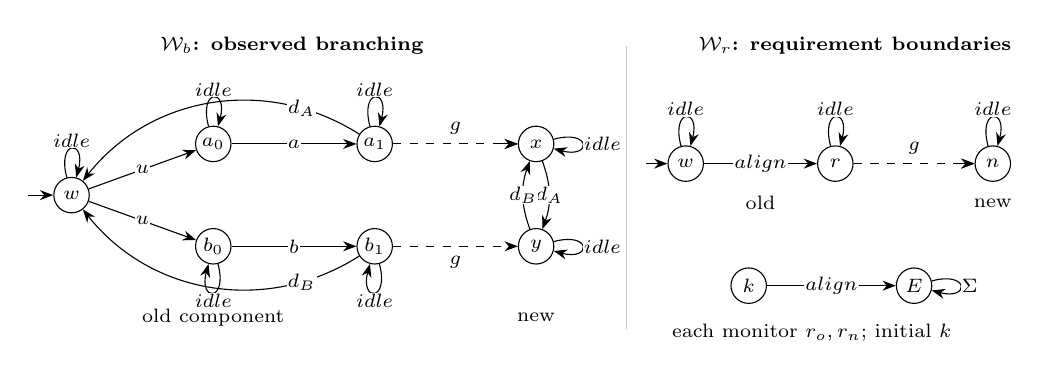
\begin{tikzpicture}[>=Stealth,every node/.style={font=\scriptsize},
 st/.style={circle,draw,minimum size=4.5mm,inner sep=1pt}]
\tikzset{labelpos/.store in=\FGpos}
\newcommand{\FGedge}[5]{\def\FGpos{.5}\draw[->,#5] (#1-#2) to node[pos=\FGpos,font=\scriptsize,fill=white,inner sep=.4pt] {$#3$} (#1-#4);}
\node[font=\scriptsize\bfseries] at (3.3,1.9) {$\mathcal W_b$: observed branching};
\node[st] (BrO-w) at (.5,0) {$w$};
\node[st] (BrO-a0) at (2.3,.65) {$a_0$};\node[st] (BrO-b0) at (2.3,-.65) {$b_0$};
\node[st] (BrO-a1) at (4.35,.65) {$a_1$};\node[st] (BrO-b1) at (4.35,-.65) {$b_1$};
\node[st] (BrN-x) at (6.4,.65) {$x$};\node[st] (BrN-y) at (6.4,-.65) {$y$};
\draw[->] (-.05,0)--(BrO-w); \draw[->] (5.85,.65)--(BrN-x);
\FGedge{BrO}{w}{u}{a0}{}
\FGedge{BrO}{w}{u}{b0}{}
\FGedge{BrO}{a0}{a}{a1}{}
\FGedge{BrO}{b0}{b}{b1}{}
\FGedge{BrO}{a1}{d_A}{w}{bend right=42,labelpos=.2}
\FGedge{BrO}{b1}{d_B}{w}{bend left=42,labelpos=.2}
\FGedge{BrO}{w}{idle}{w}{loop above}
\FGedge{BrO}{a0}{idle}{a0}{loop above}
\FGedge{BrO}{b0}{idle}{b0}{loop below}
\FGedge{BrO}{a1}{idle}{a1}{loop above}
\FGedge{BrO}{b1}{idle}{b1}{loop below}
\FGedge{BrN}{x}{d_A}{y}{bend left=20}
\FGedge{BrN}{y}{d_B}{x}{bend left=20}
\FGedge{BrN}{x}{idle}{x}{loop right}
\FGedge{BrN}{y}{idle}{y}{loop right}
\draw[->,dashed] (BrO-a1)--node[above] {$g$}(BrN-x);
\draw[->,dashed] (BrO-b1)--node[below] {$g$}(BrN-y);
\node at (2.3,-1.55) {old component};\node at (6.4,-1.55) {new};
\draw[gray!45] (7.55,1.9)--(7.55,-1.7);
\node[font=\scriptsize\bfseries] at (10.45,1.9) {$\mathcal W_r$: requirement boundaries};
\node[st] (ReqO-w) at (8.3,.4) {$w$};\node[st] (ReqO-r) at (10.2,.4) {$r$};\node[st] (ReqN-n) at (12.2,.4) {$n$};
\draw[->] (7.8,.4)--(ReqO-w);\draw[->] (11.7,.4)--(ReqN-n);
\FGedge{ReqO}{w}{align}{r}{}
\FGedge{ReqO}{w}{idle}{w}{loop above}
\FGedge{ReqO}{r}{idle}{r}{loop above}
\FGedge{ReqN}{n}{idle}{n}{loop above}
\draw[->,dashed] (ReqO-r)--node[above] {$g$}(ReqN-n);
\node at (9.25,-.1) {old};\node at (12.2,-.1) {new};
\node[st] (ReqM-k) at (9.1,-1.15) {$k$};\node[st] (ReqM-E) at (11.2,-1.15) {$E$};
\FGedge{ReqM}{k}{align}{E}{}
\FGedge{ReqM}{E}{\Sigma}{E}{loop right}
\node at (9.9,-1.75) {each monitor $r_o,r_n$; initial $k$};
\end{tikzpicture}
\par\smallskip
\fbox{\parbox{\dimexpr\linewidth-2\fboxsep-2\fboxrule\relax}{\scriptsize
Only $u$ is uncontrollable in $\mathcal W_b$; all events are controllable in $\mathcal W_r$. Arrows entering states mark local initials; dashed edges are $g$. Unlisted plant/controller transitions are empty, unlisted non-error monitor transitions self-loop, and $E$ absorbs $\Sigma$.
In $\mathcal W_b$, one-state $C^o/C^n$ loop on all six ordinary labels/$\{idle,d_A,d_B\}$; requirements are empty. In $\mathcal W_r$, one-state $C^o$ has alphabet $\{idle,align\}$ but only an $idle$ loop, and $C^n$ has only that loop; both monitors start at $k$. Supplement~S1.4 gives the complete remaining contract parameters.
}}

\caption{Finite witnesses for observation-dependent control and requirement boundaries. All ordinary transitions are shown; both contracts use the four $\Post$ rules.}
\Description{Branching witness has five old states and two new states, with all idle, uncontrollable branch and return transitions. Requirement witness has two old states and one new state; both monitors reject align. Legends specify all remaining inputs.}
\label{fig:other-witnesses}
\end{figure*}

\FloatBarrier

\begin{proposition}[Observation and requirement boundaries]
\label{prop:other-separations}
$\mathcal W_b$ has an all-root winning policy, but no fixed finite list of controllable events, whose head advances only when that event occurs and whose position is unchanged by uncontrollables, wins from $w$. $\mathcal W_r$ has a winning policy, but loses when its stop/start boundaries must form a contiguous block with no ordinary event between them; simultaneous stop/start also loses.
\end{proposition}
\begin{proof}
In $\mathcal W_b$, wait for $u$, choose $a$ or $b$ from the observed successor, then transfer; roots $a_1,b_1$ transfer immediately. The ranks of old $w$, $a_0/b_0$, $a_1/b_1$ are $3,2,1$. After $u$, the same fixed-list head faces both branches. Deleting finite $idle$ prefixes leaves a head enabled in at most one branch; an infinite idle sequence cannot finish. In $\mathcal W_r$, $t;align;s;\rho$ reaches the goal with ranks $4,3,2,1,0$. A safe $align$ must occur after $t$ and before $s$, so either boundary restriction excludes every completion. Supplement~S1 gives the full obstruction arguments and the executable-suite correspondence.
\end{proof}

\section{Certifying On-the-Fly Synthesis}
Lazy exploration solves the implicit game and produces evidence covering every entry and retained outcome, including the requirement intervals and handover targets.
\label{sec:algorithm}

\subsection{Lazy Successor Generation}

FG-DUCS-OTF instantiates the reachability attractor~\cite{Cimatti1998StrongPlanning} over typed $\Post$ with on-the-fly exploration~\cite{TripakisAltisen1999}. It queries reached-state successors in uncontrollable-first order, with lazy controllable queries, WIN serialization and exhaustive LOSS return.

The measured candidate/worklist orders are fixed in Supplement~S2. The finite candidate set $\Ev(q)\subseteq\Sigma$ is the union of local events of the active components and update events in $P$ whose precedence conditions are satisfied.
If $\Post(q,a)\neq\emptyset$, then $a\in\Ev(q)$; write its uncontrollable and controllable parts as $\Ev_{\mathrm{uc}}(q),\Ev_{\mathrm{c}}(q)$. A $\Post$ query determines contract enabledness; physical executability remains an input premise.

The algorithm maintains a discovered set $V$, an expanded set $X\subseteq V$, and a partial table
\[
 \mathcal D:\mathcal Q\times\Sigma
 \rightharpoonup 2^{\mathcal Q}\setminus\{\emptyset\}.
\tag{9}
\]
Each entry satisfies $\mathcal D(q,a)=\Post(q,a)$. For every $q\in X$, all events in $\Ev_{\mathrm{uc}}(q)$ have been queried, whereas controllable events may remain unqueried.
If no uncontrollable event is enabled, the algorithm removes and queries the first element of the fixed ordering $\Cand(q)$ of the unqueried $\Ev_{\mathrm{c}}(q)$; when the result is nonempty, it stores all successors and adds them to $V$. At all times,
$\operatorname{dom}\mathcal D\subseteq X\times\Sigma$ and
$\bigcup\operatorname{ran}\mathcal D\subseteq V$.

In the current partial table, which stores only successors enumerated by $\Post$, let the known uncontrollable results be
\[
 U_{\mathcal D}(q)=
 \bigcup_{\substack{u\in\Sigmauc\\(q,u)\in\operatorname{dom}\mathcal D}}
 \mathcal D(q,u).
\]
The winning layers of the current partial game are
\[
 W_0=V\cap\Goal,
\tag{10}\label{eq:winning-base}
\]
\[
\begin{aligned}
W_{j+1}=W_j\cup\{q\in X\setminus W_j\mid
\Safe(q)\land[
&\,U_{\mathcal D}(q)\neq\emptyset
   \land U_{\mathcal D}(q)\subseteq W_j\\
{}\lor{}&
\,U_{\mathcal D}(q)=\emptyset
   \land\exists c\in\Sigmac:
   (q,c)\in\operatorname{dom}\mathcal D
   \land\mathcal D(q,c)\subseteq W_j]\}.
\end{aligned}
\tag{11}\label{eq:winning-step}
\]
Let $W=\bigcup_{j\geq0}W_j$, and define the progress-ranking function $\rank(q)$ as the index of the first layer containing $q$.
For each $q\in W\setminus\Goal$ such that $U_{\mathcal D}(q)=\emptyset$, fix one controllable event $c_q$ satisfying
$\mathcal D(q,c_q)\subseteq W_{\rank(q)-1}$, and define, over all $\mathcal Q\setminus\Goal$,
\[
\sigma_W(q)=
\begin{cases}
\{c_q\},&q\in W\setminus\Goal\ \land\ U_{\mathcal D}(q)=\emptyset,\\
\emptyset,&\text{otherwise}
\end{cases}
\tag{12}\label{eq:sigma-construction}
\]
Thus, the policy is the fail-closed empty set at uncontrollable branches and outside $W$, and the implementation need serialize only nonempty entries.
\paragraph{Exploration invariants.}
At each loop boundary: (I1) every $q\in X$ has all uncontrollable candidates queried, including empty buckets; (I2) at LOSS return, every safe non-goal $q\in V\setminus W$ with no enabled uncontrollable has all controllable candidates queried; (I3) promotion to $W$ retains complete successor buckets and fixed lower-rank witnesses, which remain valid as $\mathcal D$ grows; and (I4) every discovered safe non-goal state outside $X$ remains in $\mathit{Open}$. Expansion completes UC queries. A retry is removed only on cursor exhaustion or promotion; added buckets cannot change retained witnesses. First discovery queues safe non-goals, and only expansion removes them. These operations preserve I1--I4; propagation is drained before either return. Supplement~S2 details the worklists.
Bucket counters and reverse incidences implement Equation~\eqref{eq:winning-step}; $r_{\rm left}=|Q_0\setminus W|$ counts uncovered roots. Duplicate-free queues and one-way cursors avoid repeated scans (Supplement~S2).

\SetAlgoNlRelativeSize{-1}
\SetAlgoRefRelativeSize{-1}
\begin{algorithm}[t]
\caption{FG-DUCS-OTF}
\label{alg:otf}
\footnotesize
\KwIn{Typed update contract (Definition~\ref{def:update_plan})}
\KwOut{$(\sigma,\rank,\kappa)$ or $(\textnormal{no solution},L)$}
$V\leftarrow Q_0$; $X,\mathcal D,\mathit{Retry}\leftarrow\emptyset$; $W\leftarrow V\cap\Goal$; $r_{\rm left}\leftarrow|Q_0\setminus W|$\;
$\mathit{Open}\leftarrow\{q\in Q_0\mid\Safe(q)\land q\notin\Goal\}$; set $\rank(q)\leftarrow0$ for $q\in W$\;
\While{true}{
  Drain the reverse-edge worklist, updating bucket counters, $(W,\rank)$, $r_{\rm left}$, and $\mathit{Retry}$\;
  \lIf{$r_{\rm left}=0$}{\Return $(\sigma,\rank|_{\Reach_\sigma(Q_0)},\kappa)$ constructed from Equations~\eqref{eq:goal} and~\eqref{eq:sigma-construction}}
  \eIf{$\mathit{Open}\neq\emptyset$}{
    Remove $q$ from $\mathit{Open}$, add it to $X$, and query all uncontrollable candidates\;
    \eIf{a nonempty uncontrollable successor set exists}{
      $\Cand(q)\leftarrow\emptyset$\;
    }{
      Set $\Cand(q)$ to the fixed-order controllable cursor; query to the next nonempty bucket or exhaustion\;
    }
    Insert $q$ into $\mathit{Retry}$ iff $q\notin W$ and $\Cand(q)\neq\emptyset$\;
  }{
    \lIf{$\mathit{Retry}=\emptyset$}{\Return $(\textnormal{no solution},L\leftarrow V\setminus W)$}
    Remove $q$ from $\mathit{Retry}$; query to the next nonempty bucket or exhaustion; reinsert iff $q\notin W$ and $\Cand(q)\neq\emptyset$\;
  }
  Enqueue each newly discovered goal for its sole $W$ insertion with $\rank=0$, or each safe non-goal in $\mathit{Open}$\;
}
\end{algorithm}
\SetAlgoNlRelativeSize{-2}
\SetAlgoRefRelativeSize{-2}

\subsection{Complexity and Static Encoding}

Let $N=|\mathcal Q|$, $A=\sum_q|\Ev(q)|$ and $B=\sum_{q,a}|\Post(q,a)|$; indexed constant-time predicates, expected-amortized constant-time dictionaries, a fixed candidate order and $O(1+|\Post(q,a)|)$ queries give $O(N+A+B)$ time and space after endpoint/eligibility preprocessing (Supplement~S2). These are explicit-game bounds: compact inputs and all-entry sets can be exponential. Java's sorting, repeated root checks and transition scans are included in the measurements; Direct-Full materializes the identical roots and terminalized game before solving it.

\begin{lemma}[Winning layers and a spoiling set]
\label{lem:attractor}
The set $W$ of Equations~\eqref{eq:winning-base}--\eqref{eq:winning-step} admits the policy of Equation~\eqref{eq:sigma-construction} and a layer rank that decreases along every successor. When no solution exists, put $L=V\setminus W$. For each safe $q\in L$, if an uncontrollable is enabled, one of its outcomes remains in $L$; otherwise, one outcome of every model-enabled controllable remains in $L$. Consequently, every state in $Q_0\cap L$ is losing.
\end{lemma}

\begin{proof}
Induction over layers shows that either all uncontrollable successors or all outcomes of the selected $c_q$ enter the preceding layer. On failure, all safe non-goal states and all necessary candidates have been expanded;
if none of the outcomes above remained in $L$, Equation~\eqref{eq:winning-step} would add $q$ to $W$. An environment policy selecting a remaining outcome either reaches an unsafe state or a deadlock,
or proceeds forever inside finite $L\setminus\Goal$; each case contradicts finite reachability.
\end{proof}

\begin{lemma}[Finite completion and rank]
\label{lem:finite-rank}
Fix a policy on a finite reachable graph, with goals terminal, safe reachable states, and nonempty successors outside $\Goal$. The following are equivalent: (i) every maximal run reaches $\Goal$; (ii) the reachable non-goal subgraph is acyclic; (iii) a natural-number rank, zero at goals and positive elsewhere, strictly decreases on every edge from a non-goal. The nonempty-successor premise excludes non-goal sinks, which would satisfy acyclicity alone.
\end{lemma}
\begin{proof}
A reachable non-goal cycle admits an infinite run. Without such a cycle, every run has at most as many non-goal steps as there are non-goal vertices; nonempty successors force it to end at a goal. The longest remaining path to a goal gives a rank, and strict rank decrease excludes every non-goal cycle.
\end{proof}

\begin{theorem}[Termination, soundness, and completeness]
\label{thm:correctness}
\label{thm:termination}
\label{thm:soundness}
\label{thm:completeness}
For every eligible finite FG-DUCS instance with Equation~\eqref{eq:nonpreemption} and quiescent goals in Equation~\eqref{eq:goal}, Algorithm~\ref{alg:otf} terminates. A returned $(\sigma,\rank,\kappa)$ satisfies every declared interval's safety relative to the supplied monitor/residual semantics and externally justified RS for $\iota_r$, preserves every uncontrollable event and every outcome of each policy event, reaches $\Goal$ finitely without deadlock, and gives each reached goal a typed-game-relative compatible target in $Z_{\mathrm{load}}$. It returns no solution iff no winning policy covers $Q_0$ in that supplied game.
\end{theorem}

\begin{proof}
\emph{Termination.} The finite input induces finitely many states and candidates. Each state is discovered and expanded at most once; each retry consumes a new candidate, and each promotion adds a state to $W$ once. Reverse incidences are processed on those promotions, so every worklist drain is finite. Eventually all roots win or both exploration queues empty.

\emph{Soundness.} Induction on winning layers gives complete retained buckets whose successors have smaller ranks: I1 supplies all uncontrollables, or the selected nonempty controllable bucket supplies all outcomes. I3 preserves this evidence. If all roots win, their policy closure is safe, has successors at every non-goal, and satisfies Lemma~\ref{lem:finite-rank}. Goal recognition uses physical quiescence and supplies each compatible $\kappa(q)$.

For interval safety, entry inherits old monitor states, initializes update monitors, and leaves new monitors inactive. An ordinary step advances exactly the active monitors. Transfer additionally changes one version and consumes its operation; stop removes its monitor before observation; start installs its supplied residual after the boundary while advancing the previously active monitors. Inactive entries remain $\bot$, and pending operations enforce one-shot execution. Induction preserves the version and activity invariants. Every retained state is non-error, so each suffix is safe for its initialized monitor; RS extends this safety to its supplied activation history. Goal matching preserves the component and new-monitor projection into the verified endpoint.

\emph{Completeness.} At failure, a root lies in $L=V\setminus W$, and $L$ contains no goal. I4 ensures every safe non-goal in $L$ was expanded. With uncontrollables, I1 and exhausted propagation imply an uncontrollable outcome in $L$; otherwise promotion would apply. Without uncontrollables, I2 gives every controllable bucket, each with an outcome in $L$ for the same reason. Against any policy, the environment keeps choosing these outcomes; permitting no event produces a deadlock. The resulting run reaches an unsafe state, deadlocks outside a goal, or remains in $L$ forever. Each contradicts winning. Hence a winning policy rules out failure; termination then forces success. Supplement~S2--S3 adds implementation-cost details and an expanded interval derivation.
\end{proof}

\begin{corollary}[Certificate checks]
\label{cor:losing}
\label{cor:independent-certificate}
Let $R_\sigma:=\Reach_\sigma(Q_0)$. A WIN certificate checks $Q_0\subseteq R_\sigma=\operatorname{dom}\rank$, safety on $R_\sigma$, and, for each $q\in R_\sigma\setminus\Goal$, $\sigma(q)\subseteq\En_{\mathrm c}(q)$, $\emptyset\neq\SuccSet_\sigma(q)\subseteq R_\sigma$, and rank decrease for every successor. It checks $\operatorname{dom}\kappa=R_\sigma\cap\Goal$ and, there, rank zero, $U(q)=\emptyset$, $\kappa(q)\in Z_{\mathrm{load}}$, and $q\sim\kappa(q)$; unserialized $\sigma$ entries are empty.
A LOSS certificate checks $L\subseteq\mathcal Q$, $Q_0\cap L\neq\emptyset$, and $L\cap\Goal=\emptyset$. Each safe $q\in L$ has an uncontrollable outcome in $L$ if one is enabled; otherwise every enabled controllable has an outcome in $L$. Unsafe states and non-goal deadlocks lose. These checks certify search results relative to shared $\Post$ and endpoint predicates~\cite{HofmannEtAl2016MuCertificates}; Section~\ref{sec:runtime-boundary} states the trust boundary.
\end{corollary}

\paragraph{Static reachability encoding.}
The environment chooses roots, uncontrollables and outcomes; otherwise the controller chooses an event. Splitting nonempty buckets through outcome vertices gives an equivalent strong-plan game in $O(N+A+B)$. Supplement~S2 proves this encoding and preservation under complete successor isomorphism; $\kappa$ remains typed endpoint evidence.
\subsection{A Separation in Successor Generation}
\begin{lemma}[Containment in full expansion]
\label{lem:full-containment}
Let both methods use identical $Q_0$, candidates, exact $\Post$, and terminal predicates, expanding neither unsafe states nor goals. Every state discovered and every bucket queried by OTF is respectively discovered and queried by Direct-Full.
\end{lemma}
\noindent The discovery-order induction, including terminal successors and query sources, is given in Supplement~S2.

\begin{theorem}[Independent updates]
\label{thm:lazy-separation}
For each $K\geq1$, there is an eligible FG-DUCS instance with $K$ independent component transfers such that Algorithm~\ref{alg:otf}, choosing a pending transfer before ordinary events, discovers exactly $K+1$ update states, whereas Direct-Full discovers $2^K$ states.
\end{theorem}
\begin{proof}
Each component has one old and one new state, related by a singleton transfer. Every version has a controllable $tick$ self-loop. The old and new controllers admit $tick$, so both endpoints are deadlock-free. There are no monitors, precedence constraints, or uncontrollables; the unique new endpoint is loadable. A state is identified by the subset $S$ of transferred components; $\rho_i$ adds $i\notin S$ and the goal is $S=I$. Every subset is reachable by performing exactly its transfers, giving $2^K$ states. Lazy expansion queries one pending transfer first at each non-goal. Serving $Open$ before $Retry$ follows one chain to the goal after $K$ steps; the next worklist drain propagates ranks $0,\ldots,K$ to the sole root before any retry. Exactly the chain's $K+1$ states are discovered. Both methods use the same quiescent terminal goal. The ordinary self-loops remain losing choices under finite completion.
\end{proof}

\section{Implementation}
\label{sec:proof}
\label{sec:runtime-boundary}

Our MTSA extension~\cite{paper:MTSA2008} implements canonical configurations, lazy buckets and certifying checks for WIN and LOSS~\cite{McConnellEtAl2011Certifying}.
\par\noindent\textbf{TCB 1---shared model semantics:} the certificate checker shares the parser, $\Post$, monitors, transfer rules, and endpoint/goal code with the synthesizer.
\par\noindent\textbf{TCB 2---checked search result:} it checks roots, safety, all outcomes, ranks/traps and handover, validating search control relative to shared semantics.
\par\noindent\textbf{TCB 3---cross-checks:} the explicit checker constructs successors separately but shares the frontend, endpoints and goal predicate. The restricted raw-LTS oracle also parses independently. Both were revised by the same author team. Residual meanings and runtime conformance remain external premises.

\paragraph{Use of generative AI}
OpenAI Codex (GPT-6 Astra; start date [要確認]) assisted contract design, semantic analysis, Java \texttt{otf} implementation/tests, campaign, rendering and analysis scripts, and figures. June--August 2026 implementation and ICSE-format drafting also used generative AI [要確認: systems/versions]. From September 14, Claude Fable 5.1 in the Anthropic desktop app assisted planning/structural diagnosis, authored the Windows driver and runbook, inspected returned raw, read source code to diagnose legacy comparisons, and drafted author decisions and task instructions. Claude authored neither manuscript prose, Java nor the renderer. ChatGPT reviewed manuscript PDFs on August 7 and September 18 [要確認: models]. Tests, raw-LTS oracles, certificate checks, primary sources and author review checked these contributions; shared authorship and AI assistance permit correlated faults. Models/logs/raw were processed locally; PDFs went to external review services. Numerical evidence uses saved outputs, not initial AI readings. Separately, Codex assisted prose drafting/revision; authors retain responsibility.

\paragraph{Runtime adapter}
A platform interprets the returned policy/rank/handover table under A1--A4. Java names entry/load \texttt{hotSwapIn}/\texttt{hotSwapOut}; the linked LTS uses an atomic goal quotient. A phase-disjoint observation map $\alpha$ must satisfy:

\noindent\textbf{A1 (endpoints):} actual endpoint observations map to same-labeled edges of $\mathsf{CL}^v$ and preserve its component and monitor states.
\textbf{A2 (update observations and progress):} at a non-goal, filtering the complete plant event set removes only controllable events outside $\sigma(q)$; every resulting event/outcome maps into $\Post(q,a)$ and is reported with its successor identity. The resulting set is nonempty and a next event is eventually observed. The latter is an execution-progress premise, independent of fairness among event choices.
\textbf{A3 (commands and observation):} commands are issued only at uncontrollable-quiescent states, finish atomically and failure-free in finite time, and report an outcome included in the supplied transfer or monitor-lifecycle rule. Internal $\tau$ steps, unobservable update outcomes, and divergence inside an update operation are outside the model: A3 requires one terminating observed command transition with its successor identity.
\textbf{A4 (boundaries):} entry atomically observes the actual reachable old state $z$ and switches to $\Init(z)$; at a quiescent goal, ordinary controllables are disabled and $\mathsf{load}$ loads $\kappa(q)$ and switches control. Each boundary is a finite, failure-free linearizable operation preserving the specified component and monitor states~\cite{HerlihyWing1990}.

\begin{theorem}[Conditional trace lifting]
\label{thm:realization}
For an eligible contract and a returned $(\sigma,\rank,\kappa)$, every execution satisfying A1--A4 lifts through $\alpha$ to the linked model. Starting at $\alpha(x_0)=\Init(z)\in Q_0$, its update segment reaches a quiescent goal within $\rank(\Init(z))$ observed update-game events and then loads the compatible endpoint through $\mathsf{load}$. Each declared active interval satisfies its supplied monitor/residual semantics, conditional on RS for the supplied initialization maps $\iota_r$. Correctness of those meanings with respect to an application's intended requirements is an input obligation.
\end{theorem}
\begin{proof}
A1 maps the old prefix to the monitored endpoint. A4 atomically maps its entry state $z$ to $\Init(z)\in Q_0$, so all-root coverage places it in the certified policy domain. Induct on observed update events. At a non-goal, A2 preserves all uncontrollables and allows only policy controllables; each reported outcome lies in its complete $\Post$ bucket. For a command, A3 supplies one finite observed transition at a quiescent source. Thus the next mapped state is a policy successor, remains in the safe certified domain, and has strictly smaller rank.

A2 supplies a next event eventually at every non-goal; neither infinite stalling nor a non-goal deadlock satisfies that premise. A natural-number rank initially $r$ permits at most $r$ decreases, forcing a goal within $r$ observed events. There, quiescence excludes an uncontrollable competitor and A4 disables ordinary controllables and performs the finite load of $\kappa(q)$. A1 maps the new continuation to its verified endpoint. The interval induction and RS in Theorem~\ref{thm:correctness} give the stated relative safety across these boundaries. Supplement~S3 expands the observation and boundary correspondence.
\end{proof}

\section{Evaluation}
\label{sec:evaluation}
We evaluate \textbf{RQ1} correctness, \textbf{RQ2} capability boundaries, \textbf{RQ3} synthesis cost on application models, and \textbf{RQ4} scaling with updates, branching and requirements.

\paragraph{Constructing the benchmark inputs.}
Nine maintained models manually adapt eight DUCS families. They declare old/new component pairs and local transfers, mainly between corresponding named states. Production Cell also maps polished states to an arm state; Railcab permits two milestone outcomes; PowerPlant leaves its initial state unmapped. The frontend generates individual stop/start events; new monitors use fluent lookup, while update monitors use a fixed post-entry state (S3). All reachable new-closed-loop states are load candidates, filtered by the goal test. No explicit precedence edges are declared (contract coverage in S4): R2 encodes selected ordering through update-time monitors; R1 monitors boundary fluents and bans specified actions. Base adds no transition requirement. Under activation-safe A, all \RSAExactNew/\RSNewOccurrences{} NEW initializers satisfy RS inclusion; equality holds when actual safe histories are nonempty. Under entry-scoped E, \RSEExactUpd/\RSUpdOccurrences{} UPD initializers are exact by the update-stage-fluent condition (S3, Lemma E$'$). The remaining \RSEUnverifiedUpd{} reference action predicates and remain unverified. H admits past violations and supplies no benchmark RS guarantee; all strict-H diagnostics remain in S4.

\paragraph{Design and measures.}
RQ3 retains all 27 instances (nine models, base/R1/R2), comparing lazy, eager-controllable, update-first, \emph{Direct-Full} and \emph{Legacy}, this fork's legacy DUCS path on the same fine-grained inputs. Legacy retains its GR objective without endpoint handover; Direct-Full uses exactly our Post/goal. On \LFFamilies{} original DUCS models and \LFConditions{} monolithic conditions, a lab-maintained build of the original DUCS source returns \LFPublishedWins{} controllers; the aligned fork agrees on all \LFForkWins{} jointly processed conditions, with \LFSizeMatches{} matching first-trial sizes and a \LFRailcabStateDelta{}-state Railcab difference amid repetition variation (Supplement~S4). The remaining \LFUnmeasured{} stop before a legacy GR decision (\LFParserNM{} parser, \LFInstrumentationNM{} instrumentation), providing no evidence of legacy synthesis failure. Capability separations use RQ2 witnesses.

Trials run sequentially on Windows~10, Xeon W-2265, 256~GB RAM, Temurin~17.0.20.1, with a 64~GiB heap and 1,200~s limit. Stage~1 covers all 135 RQ3 pairs. Valid decisions receive four further runs; failures are retained without repetition. Medians and min--max require five valid, consistent completions. An authorized same-setting Workflow/R2 Direct-Full supplement times out at \ADWorkflowCapSeconds{}~s; the original operational interruption is retained in S4. A separate \ADPCCapSeconds{}~s PC Arms=2/R2 FG trial also times out and contributes no median.

We record states, queries, transitions, solver time, sampled peak JVM RSS and policy size. LTS time includes checking; hub is solve-only; Legacy uses its native timer. Endpoint/process times are separate. Completed-pair ratios use solver intervals, excluding frontend/startup; S4 also reports total JVM elapsed time. Mac pilot times are excluded.

\subsection{RQ1: Correctness}
\textbf{Answer.} All 92 jobs agree with independently derived raw-LTS expectations (Table~\ref{tab:rq1-validation}). Cases cover semantic boundaries, related variants and endpoint contracts, including missing controller events, deadlocks and suppressed uncontrollables (S4).

\begin{table}[!htbp]
\caption{Local validation of the confirmed semantics, separate from Xeon cost measurements. Counts are jobs; variants share source models.}
\label{tab:rq1-validation}
\centering\small
\begin{tabular}{@{}lrrrrl@{}}
\toprule
Stratum & Jobs & WIN & LOSS & Invalid & Expected agreement\\
\midrule
Semantic models, two methods & 82 & 34 & 48 & 0 & 82/82\\
Endpoint contracts, two methods & 10 & 2 & 0 & 8 & 10/10\\
\textbf{RQ1 total} & \textbf{92} & \textbf{36} & \textbf{48} & \textbf{8} & \textbf{92/92}\\
\bottomrule
\end{tabular}
\end{table}

The Python oracle independently parses restricted FSP and derives synchronous graphs, ranks and losing closure. Separate probes confirm transfer-blocking old UC loops, new UC loops changing WIN to LOSS, and quiescence after a finite UC suffix.

All eligible jobs pass certificates and separate exhaustive checks; every WIN passes atomic Link. Section~\ref{sec:runtime-boundary} states the trust boundary; S4 gives denominators and test counts.

\subsection{RQ2: Capability}
\textbf{Answer.} Fine-grained policies win where each tested restriction loses: eight LTS files yield ten WIN and four LOSS, all matching independent expectations (Table~\ref{tab:capability-revalidated}). They test the cell obstruction, both fixed heads, contiguous boundaries and neutral controls (S1). Industry/R1's checked LOSS rejects its supplied contract; it is not a capability separation.

\begin{table}[!htbp]
\caption{Completed formal capability checks. W/L counts winning/losing jobs. Both fixed resolving heads are tested.}
\label{tab:capability-revalidated}
\centering\small
\begin{tabular}{@{}llrr@{}}
\toprule
Witness & Policy/model & Separation W/L & Neutral W/L\\
\midrule
Production Cell & Local transfer & 1/0 & 1/0\\
 & Simultaneous transfer & 0/1 & 1/0\\
Observed branch & Full policy & 1/0 & 1/0\\
 & Fixed heads & 0/2 & 2/0\\
Requirement boundary & Interleaved & 1/0 & 1/0\\
 & Contiguous block & 0/1 & 1/0\\
\bottomrule
\end{tabular}
\end{table}

\subsection{RQ3: Synthesis Cost}
\textbf{Answer.} Within the fixed budget, lazy decides more instances; its completed Direct-Full pairs agree and are faster. Table~\ref{tab:xeon-rq3} retains all 135 cells. Lazy synthesis returns 25 WIN, one LOSS (Industry/R1), and one TO (PC Arms=2/R2). Direct-Full returns \ADDirectFullWins{} WIN and \ADDirectFullTimeouts{} TO, including the marked supplement. Their 14 completed decisions agree; Direct-Full/FG ratios of five-run median solver times range from $1.58$ to $2{,}123.81$, with median $9.14$. These are paired costs, not realizability separations. For \CensoredPairs{} DF timeouts with completed FG runs, censored JVM-attempt/FG elapsed-median lower bounds span \CensoredBoundMin--\CensoredBoundMax{} (S4); these bounds cover total time, not solver time. PC Arms=2/R2 remains unresolved after \ADPCCapSeconds{}~s, with \ADPCPeakRSSGiB{}~GiB peak process RSS under the 64~GiB heap cap.

Candidate orders and Open/Retry ties are fixed in S2; eager and update-first test sensitivity to order and materialization. Eager-controllable decides 17 instances; update-first decides 24 (23 WIN, one LOSS), versus lazy's 26. All paired decisions agree; update-first is faster on 8/24 pairs. Legacy has nine WIN agreeing with FG, 13 OOM and five N/M (capture cap). The author-side cap prevents measurement before synthesis, evidencing no Legacy failure. Its GR objective and native timer delimit this reference comparison.

Industry/R1 loses at 42 of 131 entries: the FG contract requires every entry to force quiescent handover to a verified new-controller state. Separate exhaustive checking confirms the losing region: after all nine updates, an incompatible state admits repeated DSD1 rejection, while R1 prevents earlier history repair (Supplement~S4). By contrast, a lab-maintained build of the original DUCS source returns a 2,312-state monolithic controller under \texttt{T\_Empty} for the source model of the fine-grained adaptation, as does the fork once entry labels are aligned. Published DUCS continues control under the new specification without requiring a preverified new-controller connection~\cite[Defs.~4.1--4.3]{Nahabedian2020}. This LOSS is specific to the supplied FG contract.

Exempting only \texttt{validateGF1} from the three R1 bans makes all 131 roots WIN with certificate, Link and exhaustive checks, keeping other inputs and Post/goal fixed. This Mac contract variant assumes validation is acceptable during update and is excluded from Table~\ref{tab:xeon-rq3} (S4).

\begin{table}[!htbp]
\caption{RQ3 solver time (seconds), all 27 instances and five methods. Medians require five valid, consistent completions; other cells retain statuses. PC Arms=1 is the DUCS Production Cell benchmark; Arms=2 is its extension included in the 27 instances since the ICSE draft. Ranges and full metrics: Supplement~S4.}
\label{tab:xeon-rq3}
\centering
\begingroup\scriptsize\setlength{\tabcolsep}{3pt}
\begin{tabular}{@{}llccccc@{}}
\toprule
Model & Req. & FG lazy & Eager & Update-first & Direct-Full & Legacy\\
\midrule
GSM & BASE & W 0.0224$^{\dagger}$ & W 0.0332$^{\dagger}$ & W 0.0233 & W 0.0416 & W 0.241\\
 & R1 & W 0.0228 & W 0.0348$^{\dagger}$ & W 0.0243 & W 0.045 & W 0.306\\
 & R2 & W 0.0201$^{\dagger}$ & W 0.0281 & W 0.0225 & W 0.0327$^{\dagger}$ & W 0.25\\
\addlinespace[2pt]
Industry & BASE & W 0.19 & W 14.5 & W 0.542 & W 154 & N/M\\
 & R1 & L 562 & TO & L 461$^{\dagger}$ & TO & N/M\\
 & R2 & W 1.15 & W 2.96 & W 0.455 & W 28 & N/M\\
\addlinespace[2pt]
MetaSocket & BASE & W 0.0149$^{\dagger}$ & W 0.0302$^{\dagger}$ & W 0.0165$^{\dagger}$ & W 0.0408 & W 0.323\\
 & R1 & W 0.0136$^{\dagger}$ & W 0.0278$^{\dagger}$ & W 0.0147 & W 0.0426$^{\dagger}$ & W 0.443\\
 & R2 & W 0.0152$^{\dagger}$ & W 0.018 & W 0.0154$^{\dagger}$ & W 0.024$^{\dagger}$ & W 0.29\\
\addlinespace[2pt]
PowerPlant & BASE & W 0.0463$^{\dagger}$ & W 0.487 & W 0.052 & W 1.85 & W 18$^{\dagger}$\\
 & R1 & W 0.125$^{\dagger}$ & W 1.08 & W 0.152 & W 5.51 & W 896$^{\dagger}$\\
 & R2 & W 0.18 & W 0.251 & W 0.114 & W 1.01 & W 8.25\\
\addlinespace[2pt]
PC Arms=1 & BASE & W 0.0741$^{\dagger}$ & W 26 & W 0.886 & W 157 & N/M\\
 & R1 & W 0.0793 & W 188 & W 3.15 & TO & OOM\\
 & R2 & W 6.16$^{\dagger}$ & W 12.2 & W 1.17 & W 77.8 & N/M\\
\addlinespace[2pt]
PC Arms=2 & BASE & W 2.61$^{\dagger}$ & TO & TO & TO & OOM\\
 & R1 & W 2.6 & TO & TO & TO & OOM\\
 & R2 & TO\textsuperscript{a} & TO & TO & TO & OOM\\
\addlinespace[2pt]
Railcab & BASE & W 0.169 & TO & W 2.26 & TO & OOM\\
 & R1 & W 3.18 & TO & W 6.74 & TO & OOM\\
 & R2 & W 15.5 & W 38.7 & W 4.16 & W 283 & OOM\\
\addlinespace[2pt]
Surveillance & BASE & W 2.01 & TO & W 2.63$^{\dagger}$ & TO & OOM\\
 & R1 & W 18.6 & TO & W 126 & TO & OOM\\
 & R2 & W 37.1 & TO & W 16.1 & TO & OOM\\
\addlinespace[2pt]
Workflow & BASE & W 0.111 & W 508 & W 0.116 & TO & OOM\\
 & R1 & W 0.325 & TO & W 0.215 & TO & OOM\\
 & R2 & W 16.1 & W 23.9 & W 3.18 & TO$^{\ddagger}$ & OOM\\
\addlinespace[2pt]
\bottomrule
\end{tabular}\endgroup
\par\smallskip{\scriptsize W/L: winning/losing. Seconds: median only for five valid, consistent completions; ranges in S4. TO: 1,200 s timeout; OOM: out of memory. N/M (capture cap): author-side M9MtsSnapshot instrumentation stops before synthesis at its fixed 250,000-state cap; no evidence of Legacy capability or solver failure. Original operational interruptions are retained in S4. Legacy uses native semantics. Other incomplete groups show statuses, without medians. $\dagger$: $(\max-\min)/\mathrm{median}>10\%$ (also a zero median with a positive range); see Supplement~S4.}\par{\scriptsize $^{a}$ The separate 3,600 s single trial also timed out (peak process RSS 67.1 GiB; 64 GiB heap cap). $^{\ddagger}$ The original trial was operationally interrupted; the pre-authorized same-setting replacement timed out at 1,200 s. Both records remain in Supplement~S4. RSS does not establish heap saturation.}

\end{table}

\subsection{RQ4: Scaling}
\textbf{Answer.} Lazy exploration reduces cost along the independent-update and tested hub axes, while Travel retains a shared concurrency limit. All four methods finish independent updates for $K=2,\ldots,20$ (Figure~\ref{fig:xeon-scaling}). At $K=20$, lazy and update-first discover 21 states, eager 211, and Direct-Full $1{,}048{,}576$. Their five-run median times are respectively 0.0354, 0.0318, 0.0625 and 853~s. The exact separation concerns this constructed family.

Across 33 controlled instances (132 single-run jobs), every method returns 31 WIN and two LOSS. With eight monitors, lazy discovers 18 states versus Direct-Full's $1{,}179{,}640$; larger transfer fanout forces every method to retain all outcomes (S4; no timing medians).

Travel retains all 48 $(N,K)$ instances in Figure~\ref{fig:xeon-scaling}. Lazy, eager and update-first each finish 20; Direct-Full finishes 18. On 18 completed pairs, lazy uses 3.4--46.2\% of Direct-Full's states; median-time ratios are $1.49$--$34.21$ (median $3.93$). Lazy and update-first match states, queries and outcomes on all 20 completions. All methods remain unresolved at $N=4,K\geq8$ and every tested $N\geq6$ (1,200~s/64~GiB): lazy exploration benefits the $K$ axis but leaves a shared concurrency limit.

All 90 hub instances (30 seeds, three UC profiles, $n=4$) finish five repetitions per method with agreeing decisions. Direct-Full/lazy ratios are $5.35$--$118.38$ (median $78.11$); lazy's largest median is 0.918~s. Each seed/profile is plotted separately.

\begin{figure}[!htbp]
\centering
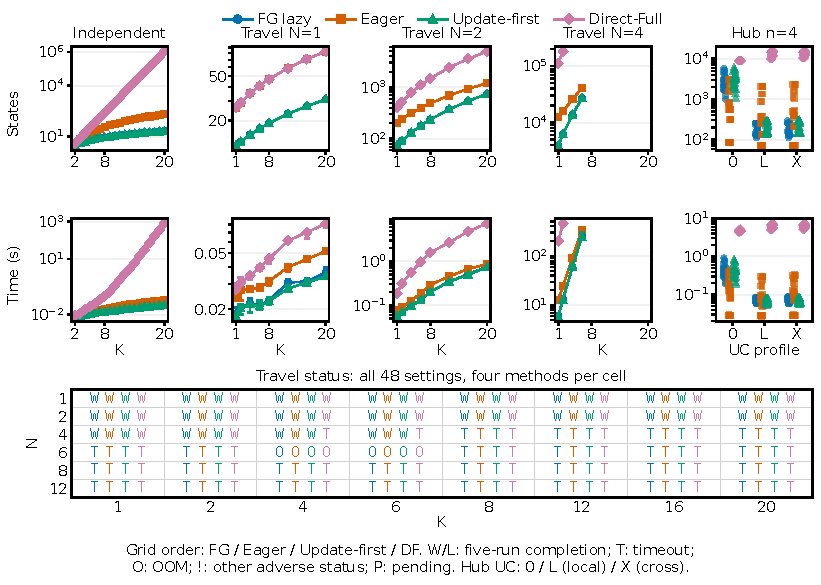
\includegraphics[width=\linewidth]{build/generated/rq4-scaling-combined.pdf}
\caption{RQ4 first-trial discovered states (top) and five-run median solver time with min--max (middle). Hub uses solve-only time, plotting every seed/profile. The bottom grid retains all 48 Travel settings and four methods, including TO/OOM; incomplete cells have no timing median. Full panels: Supplement~S4.}
\Description{Five columns show independent updates, Travel N=1, 2 and 4, and hub profiles. A six-row status grid also retains Travel N=6, 8 and 12 with all tested K values and method statuses.}
\label{fig:xeon-scaling}
\end{figure}

\subsection{Threats to Validity}
\label{sec:threats}
Checkers, tests and code share the author team and AI assistance, allowing correlated faults. The raw oracle supports a restricted language. A establishes RS inclusion for all \RSAExactNew/\RSNewOccurrences{} NEW initializers; equality needs nonempty actual safe histories, whose plant-level nonemptiness is unverified. E certifies \RSEExactUpd/\RSUpdOccurrences{} UPD initializers; the remaining \RSEUnverifiedUpd{} reference action predicates and need entry-value-dependent language checks. H supplies no benchmark RS guarantee. A1--A4 and runtime loading need validation. Nine adaptations of eight families are correlated cases, not independent samples; interpretation is by family. Constructed witnesses limit generalization. Legacy denotes our fork; its GR objective differs from FG. It does not process \LFUnmeasured/\LFConditions{} original inputs accepted by the lab build; one first-trial size differs, and sizes vary across repetitions (Supplement~S4).

Timings select completed pairs; all 135 cells retain unresolved outcomes. The author-side capture cap prevents measurement, implying no Legacy failure. Update-first wins some timing pairs. Industry/R1's LOSS and validation-permitting WIN depend on the contract. Sampled RSS can miss peaks. One machine, heap and synthetic families limit generalization; all methods remain unresolved on Travel at every tested $N\geq6$. PC Arms=2/R2 remains unresolved at \ADPCCapSeconds{}~s; S4 preserves both original and supplementary records. Earlier adverse results and old-goal checks remain archived outside current measurements.

\section{Related Work}
\label{sec:expressiveness}
FG-DUCS inherits established reachability attractors and OTF exploration~\cite{Cimatti1998StrongPlanning,TripakisAltisen1999,CiolekEtAl2023OTFDCS}, the DUCS update-control problem~\cite{Nahabedian2020}, and trace-dependent residual obligations from Live Synthesis~\cite{FinkbeinerEtAl2022LiveSynthesis}. FG combines nondeterministic component transfers, individual requirement boundaries and $\iota$ under RS, precedence, $Z_{load}$ and quiescent goals, with finite completion for all entries and outcomes, no fairness, and WIN/LOSS evidence. Table~\ref{tab:closest-native} compares native contracts; marked-state nonblocking instead permits an existential completing continuation.

\begin{table*}[!htbp]
\caption{Primary-source contracts and progress premises (UC: uncontrollable). Full comparison: Supplement~S5.}
\label{tab:closest-native}
\centering\footnotesize
\setlength{\tabcolsep}{3pt}\renewcommand{\arraystretch}{1.02}
\begin{tabular}{@{}>{\raggedright\arraybackslash}p{.16\linewidth}>{\raggedright\arraybackslash}p{.34\linewidth}>{\raggedright\arraybackslash}p{.46\linewidth}@{}}
\toprule
Work & Update/control contract & Roots, outcomes and progress\\
\midrule
DUCS~\cite{Nahabedian2020,Nahabedian2016SEAMS}
& Global environment/spec switch; set-valued transfer; order formula $T$
& All old states/outcomes; eventual update after hotSwap; legal, deadlock-free (Defs.~4.1--4.3)\\
GR(1) bridge~\cite{Amram2022GR1DynamicUpdate}
& Old safety before switch, new spec afterward
& All prefixes meeting new environment safety; bounded switch (Def.~3.1); later liveness assumes justice\\
Live Synthesis~\cite{FinkbeinerEtAl2022LiveSynthesis}
& Old/new LTL; residual $\Psi(\eta,\varphi)$
& Universal: all old prefixes/new traces; old obligations finitely satisfied, one eventual update (Thm.~6.4)\\
DES state attraction~\cite{NooruldeenSchmidt2015}
& Common deterministic plant; task recognizer
& All requests; UC preserved; weakly invariant startup; bounded first completion (Def.~2, Thm.~1)\\
OTF-DCS~\cite{CiolekEtAl2023OTFDCS}
& Components, marked/illegal states, control partition
& All UC; designated disturbances; eager director (Def.~3); every prefix has a marked extension (Def.~4)\\
Dynamic Feature~\cite{ThuijsmanReniers2024DynamicFeature}
& Feature changes, reinitialization, configuration/behavior constraints
& Mixed control; every reachable state has a jointly marked continuation (Sec.~7)\\
\bottomrule
\end{tabular}
\end{table*}

DUCS exposes global reconfiguration, whole-set stop/start and set-valued transfers; stages can be encoded in the new environment~\cite[Sec.~4.2, Defs.~4.1--4.2]{Nahabedian2020}. Individual boundaries and residuals then require explicit mode/history encoding rather than native inputs. Direct-Full measures explicit expansion of the same FG $\Post$/goal, not a translated DUCS implementation.

The GR(1) bridge preserves old safety, without old justice, until a bounded switch under new environment safety; new justice assumes environment justice~\cite[Def.~3.1]{Amram2022GR1DynamicUpdate}. FG adds individual residuals, transfer outcomes, quiescent boundaries and all-root coverage.

DES state attraction bounds completion on a deterministic plant with a weakly UC-invariant startup set~\cite[Def.~2, Thm.~1]{NooruldeenSchmidt2015}. FG instead quantifies over all roots and transfer outcomes in a mode/residual product with compatible quiescent targets.

OTF-DCS~\cite[Defs.~3--4]{CiolekEtAl2023OTFDCS} explores component-based directed control: each prefix needs a completing extension, whereas every FG continuation must complete handover.

Scenario, process, workflow and UAV updates preserve obligations~\cite{Ghezzi2012DynamicScenarioUpdate,PanzicaLaManna2013CorrectnessDynamicUpdates,NahabedianEtAl2022Business,Sokolowski2022DynamicWorkflowUpdates,ZudaireEtAl2022UAV}; evolving monitors carry history~\cite{CarwehlEtAl2023ChangingRequirements,KristensenEtAl2026DynSRV}. Reconfiguration and lifecycle methods coordinate control, structure and replacement~\cite{DelavalRutten2010Reconfiguration,KhakpourArbabRutten2016Reconfiguration,BresolinLanese2021PropertyPreservingUpdates,DiCosmoEtAl2014Aeolus,ChardetEtAl2021Concerto,RobillardCoullon2022Planning}; network updates address state transfer and stages~\cite{SaurEtAl2016Morpheus,McClurgEtAl2015NetworkUpdates,QiuEtAl2023FlexPlan}. FG requires all-outcome completion at a verified endpoint.

\FloatBarrier
\section{Conclusion}
\label{sec:conclusion}

FG-DUCS certifies all-root, all-outcome completion or failure relative to the supplied finite model and RS, with execution guarantees under A1--A4. A establishes RS inclusion for all \RSAExactNew{} NEW initializers, with equality on nonempty safe histories. E certifies \RSEExactUpd/\RSUpdOccurrences{} UPD initializers; \RSEUnverifiedUpd{} remain unverified. Lazy synthesis decides 26/27 Xeon instances versus Direct-Full's 14, with paired speedups of $1.6$--$2{,}124\times$; hub yields $5.3$--$118\times$. Travel's shared resource limits, the certified LOSS and unresolved outcomes delimit the empirical results.

\clearpage
\paragraph{Data Availability.}
The anonymous repository~\cite{FGDUCSAnonymousArtifact} provides the complete MTSA-derived tool sources, FG-DUCS extensions, models, scripts, RQ1/RQ2 evidence and supplement. It also provides generated tables, inputs and diffs for Xeon RQ3, all RQ4 families, both RQ3 supplementary campaigns and the separate monolithic legacy-fidelity reference results. Larger raw outputs are packaged as two verified split assets; their publication in the \texttt{v2-preview} pre-release is pending. The submission version is designated \texttt{fse27-submission}; this tag will be created after v2 is frozen. A public HTTPS clean clone, empty-cache source build and RQ1/RQ2 derive-only checks have passed; public asset restoration awaits the Release. Included scripts fetch third-party dependencies from official upstream distributions; the shaded JAR is not distributed. Checker-pass records and serialized bodies are distinguished, and personal paths anonymized.

\bibliographystyle{ACM-Reference-Format}
\bibliography{references}

\end{document}
